\section{1174091 - Alfadan Owen}
\subsection{Teori}
\begin{enumerate}

	\item Jelaskan apa itu klasifikasi teks, sertakan gambar ilustrasi buatan sendiri.
	\hfill\break
	Klasifikasi teks merupakan salah satu tugas terpenting dalam Pemrosesan Bahasa Alami (Natural Language Processing). Ini adalah proses mengklasifikasikan string teks atau dokumen ke dalam kategori yang berbeda, tergantung pada konten string. Klasifikasi teks memiliki berbagai aplikasi, seperti mendeteksi sentimen pengguna dari tweet, mengklasifikasikan email sebagai spam atau ham, mengklasifikasikan posting blog ke dalam kategori yang berbeda, penandaan otomatis permintaan pelanggan, dan sebagainya. Berikut adalah contoh dari Klasifikasi Teks. Contohnya, misal kita ingin mencari kata dog, table, on, the . kemudian jika kata yang dimaksud sesuai maka akan menampilkan bilangan biner 1 dan jika salah 0. 
	\begin{figure}[H]
	\centering
		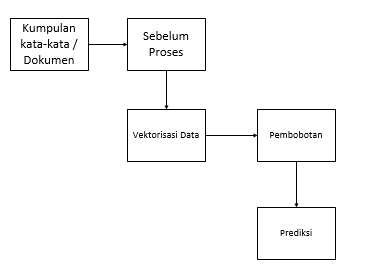
\includegraphics[width=7cm]{figures/1174091/4/1.png}
		\caption{Klasifikasi teks}
	\end{figure}
	
	\item Jelaskan mengapa Klasifikasi bunga tidak bisa menggunakan machine learning, sertakan ilustrasi sendiri.	
	\hfill\break
	Dikarenakan tidak semua bunga memliki ciri - ciri yang sama. Atau dalam kata lain terdapat data noise dalam klasifikasi bunga sehingga tidak bisa menggunakan machine learning. Contohnya Anggrek memiliki warna ungu, dengan jumlah kelopak 5. Kemudian ada bunga warna ungu dengan jumlah kelopak yang sama namun ternyata bukan anggrek dan kategorinya banyak sekali. Bahkan ada bunga yang tidak jelas apakah warnanya sesuai atau tidak, sehingga bisa menyebabkan data noise.

	\begin{figure}[H]
	\centering
		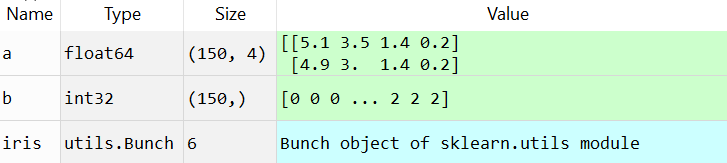
\includegraphics[width=7cm]{figures/1174091/4/2.png}
		\caption{Klasifikasi Bunga}
	\end{figure}

	\item Jelaskan bagaimana teknik pembelajaran mesin pada teks pada kata-kata yang digunakan di youtube,jelaskan arti per atribut data csv dan sertakan ilustrasi buatan sendiri.

	Menggunakan teknik bag-of-words pada klasifikasi berbasis text dan kata untuk mengklasifikasikan komentar yang ada di internet sebagai spam atau bukan. Misalkan pada kolom komentar dapat di cek seberapa sering suatu kata muncul dalam kalimat. Setiap kata dapat dijadikan baris dan kolomnya ini merupakan kategori kata terbut, apakah masuk kedalam spam atau tidak. dan contoh lainnya yaitu pada Caption. dimana akan muncul subtitle secara otomatis dari youtube menggunakan sensor suara yang disesuaikan degan kata yang telah ditentukan
	\begin{figure}[H]
	\centering
		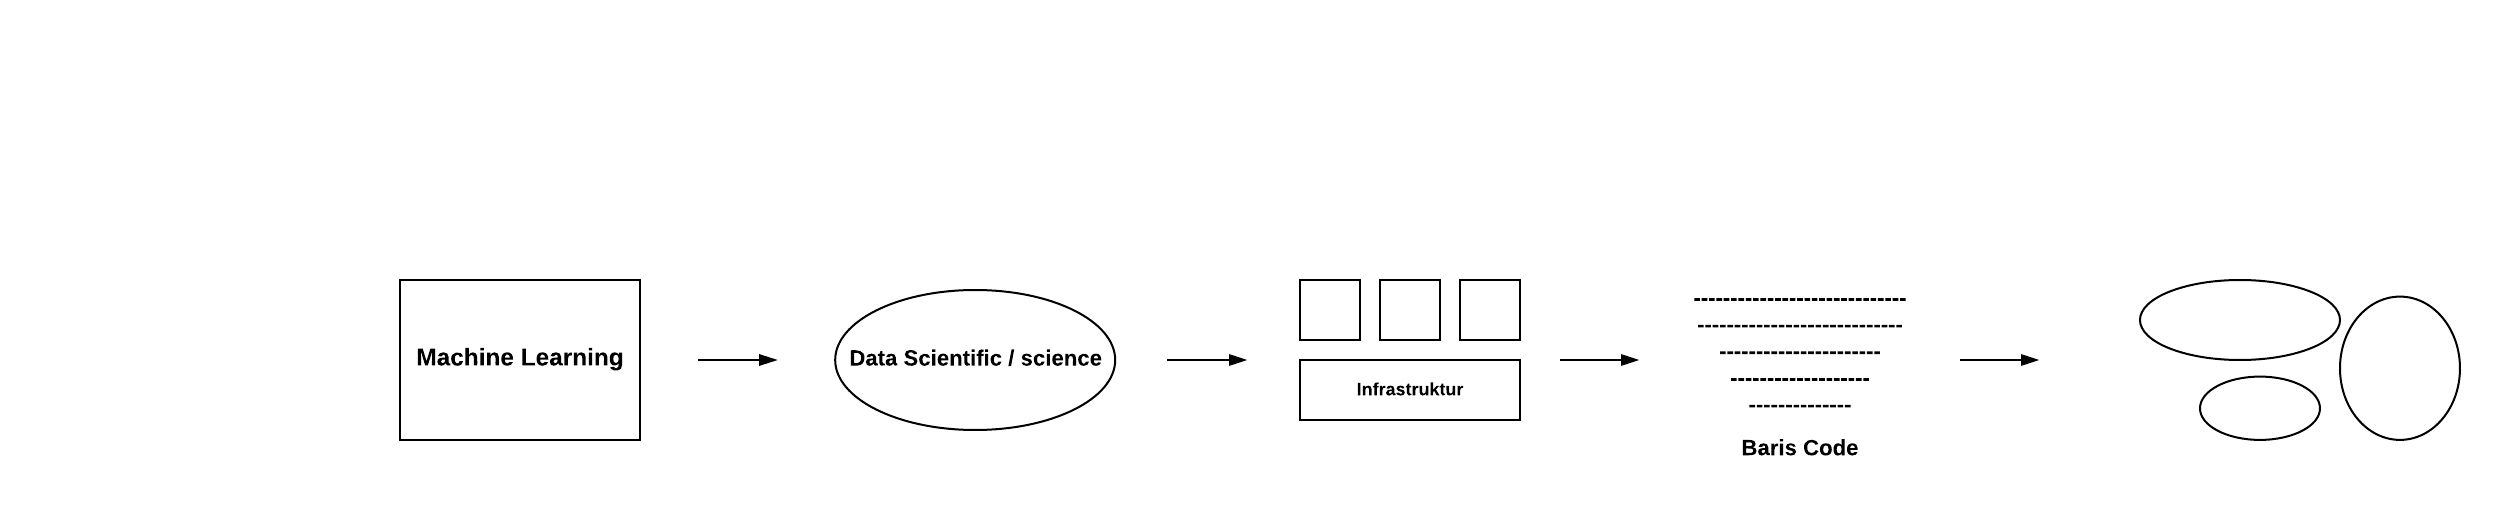
\includegraphics[width=7cm]{figures/1174091/4/3.png}
		\caption{Klasifikasi Bunga}
	\end{figure}

	\item Jelaskan apa yang dimaksud vektorisasi data.
	\hfill\break
	Vektorisasi adalah proses konversi data raster menjadi data vektor yang lebih umum disebut dengan istilah digitalisasi adapun aktifitasnya disebut digitasi. Wujud digitalisasi ini diklasifikasikan secara spesifik dalam tema-tema tertentu yang direpresentasikan oleh bentuk garis, poligon dan titik. Pada akhirnya proses vektorisasi ini menghasilkan suatu wujud peta topografi yang menggambarkan keadaan permukaan bumi atau bentang alam. Sifat data yang geometris menunjukkan ukuran dimensi yang sesungguhnya. 

	\item Jelaskan apa yang dimaksud dengan bag of words dengan ilustrasi sendiri.
	\hfill\break
	Bag of Words Merupakan representasi teks yang menggambarkan kemunculan kata-kata dalam dokumen. ePngelompokan kata kata kedalam perhitunga, berapakali sebuah kata muncul dalam satu kalimat. Disebut ”tas” kata-kata, karena informasi tentang susunan atau struktur kata dalam dokumen dibuang. Model ini hanya berkaitan dengan apakah kata-kata yang diketahui muncul dalam dokumen, bukan di mana dalam dokumen.
	Contohnya disini akan melihat kemunculan kata dari kalimat :
1. I love hashinshin
2. I hate tyler1
3. hashinshin rage quit

	\begin{figure}[H]
	\centering
		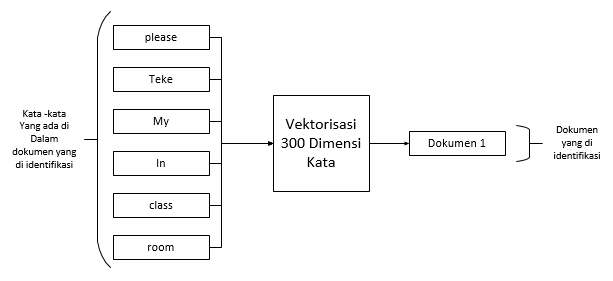
\includegraphics[width=7cm]{figures/1174091/4/4.png}
		\caption{Bag of words}
	\end{figure}

	\item Jelaskan apa yang dimaksud dengan TF-IDF.
	\hfill\break
	TF-IDF memberi kita frekuensi kata dalam setiap dokumen dalam korpus atau mengganti data jadi number. Ini adalah rasio berapa kali kata itu muncul dalam dokumen dibandingkan dengan jumlah total kata dalam dokumen itu. Itu meningkat seirin jumlah kemunculan kata itu di dalam dokumen meningkat. Setiap dokumen memiliki tf sendiri. Dalam ilustrasi disini saya akan mengganti contoh Bag of Words menjadi bentuk TF-IDF.
1. I love dogs
2. I hate dogs and knitting
3. knitting is my hobby and passion


	\begin{figure}[H]
	\centering
		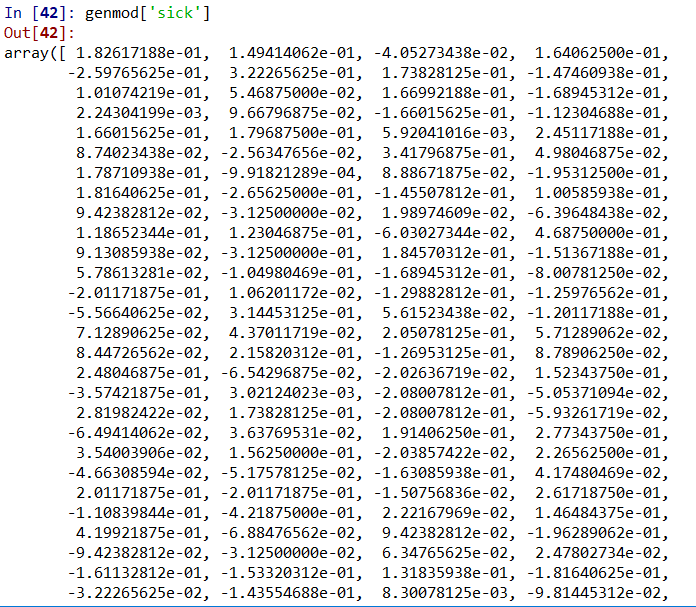
\includegraphics[width=7cm]{figures/1174091/4/5.png}
		\caption{TF-IDF}
	\end{figure}
\end{enumerate}


\subsection{Praktek Program}
\begin{enumerate}
	\item Soal 1
	\hfill\break
	\lstinputlisting[firstline=8, lastline=9]{src/1174091/4/1174091.py}
	Kode di atas digunakan untuk buat aplikasi sederhana menggunakan pandas dengan format csv sebanyak 500 baris  
	
	\item Soal 2
	\hfill\break
	\lstinputlisting[firstline=11, lastline=12]{src/1174091/4/1174091.py}
	Kode di atas digunakan untuk memecah dataframe tersebut menjadi dua bagian yaitu 450 row pertama dan 50 row kedua. Hasilnya adalah sebagai berikut 

	\item Soal 3
	\hfill\break
	\lstinputlisting[firstline=9, lastline=9]{src/1174091/4/1174091-2.py}
	Dengan menggunakan 1174091 mod 4 adalah 3, yang artinya menggunakan dataset shakira. 
		

	\item Soal 4
	\hfill\break
	\lstinputlisting[firstline=12, lastline=36]{src/1174087/4/1174087.py}
	Klasifikasi dari data vektorisasi menggunakan klasifikasi SVM.
	

	\item Soal 5
	\hfill\break
	\lstinputlisting[firstline=40, lastline=43]{src/1174091/4/1174091-2.py}
	Klasifikasi dari data vektorisasi menggunakan klasifikasi Decision Tree.
	

	\item Soal 6
	\hfill\break
	\lstinputlisting[firstline=60, lastline=106]{src/1174091/4/1174091-2.py}
	Plot confusion matrix dari praktik modul ini menggunakan matplotlib. 

	\item Soal 7
	\hfill\break
	\lstinputlisting[firstline=214, lastline=224]{src/1174091/4/1174091-2.py}
	Menjalankan program cross validation. 

	\item Soal 8
	\hfill\break
	\lstinputlisting[firstline=227, lastline=241]{src/1174091/4/1174091-2.py}
	Program pengamatan komponen informasi. Jadi disini kita akan memprediksi nilai dari variabel test att dan test pass 

